% Options for packages loaded elsewhere
\PassOptionsToPackage{unicode}{hyperref}
\PassOptionsToPackage{hyphens}{url}
\PassOptionsToPackage{dvipsnames,svgnames,x11names}{xcolor}
%
\documentclass[
  letterpaper,
  DIV=11,
  numbers=noendperiod]{scrartcl}

\usepackage{amsmath,amssymb}
\usepackage{iftex}
\ifPDFTeX
  \usepackage[T1]{fontenc}
  \usepackage[utf8]{inputenc}
  \usepackage{textcomp} % provide euro and other symbols
\else % if luatex or xetex
  \usepackage{unicode-math}
  \defaultfontfeatures{Scale=MatchLowercase}
  \defaultfontfeatures[\rmfamily]{Ligatures=TeX,Scale=1}
\fi
\usepackage{lmodern}
\ifPDFTeX\else  
    % xetex/luatex font selection
\fi
% Use upquote if available, for straight quotes in verbatim environments
\IfFileExists{upquote.sty}{\usepackage{upquote}}{}
\IfFileExists{microtype.sty}{% use microtype if available
  \usepackage[]{microtype}
  \UseMicrotypeSet[protrusion]{basicmath} % disable protrusion for tt fonts
}{}
\makeatletter
\@ifundefined{KOMAClassName}{% if non-KOMA class
  \IfFileExists{parskip.sty}{%
    \usepackage{parskip}
  }{% else
    \setlength{\parindent}{0pt}
    \setlength{\parskip}{6pt plus 2pt minus 1pt}}
}{% if KOMA class
  \KOMAoptions{parskip=half}}
\makeatother
\usepackage{xcolor}
\setlength{\emergencystretch}{3em} % prevent overfull lines
\setcounter{secnumdepth}{-\maxdimen} % remove section numbering
% Make \paragraph and \subparagraph free-standing
\makeatletter
\ifx\paragraph\undefined\else
  \let\oldparagraph\paragraph
  \renewcommand{\paragraph}{
    \@ifstar
      \xxxParagraphStar
      \xxxParagraphNoStar
  }
  \newcommand{\xxxParagraphStar}[1]{\oldparagraph*{#1}\mbox{}}
  \newcommand{\xxxParagraphNoStar}[1]{\oldparagraph{#1}\mbox{}}
\fi
\ifx\subparagraph\undefined\else
  \let\oldsubparagraph\subparagraph
  \renewcommand{\subparagraph}{
    \@ifstar
      \xxxSubParagraphStar
      \xxxSubParagraphNoStar
  }
  \newcommand{\xxxSubParagraphStar}[1]{\oldsubparagraph*{#1}\mbox{}}
  \newcommand{\xxxSubParagraphNoStar}[1]{\oldsubparagraph{#1}\mbox{}}
\fi
\makeatother

\usepackage{color}
\usepackage{fancyvrb}
\newcommand{\VerbBar}{|}
\newcommand{\VERB}{\Verb[commandchars=\\\{\}]}
\DefineVerbatimEnvironment{Highlighting}{Verbatim}{commandchars=\\\{\}}
% Add ',fontsize=\small' for more characters per line
\usepackage{framed}
\definecolor{shadecolor}{RGB}{241,243,245}
\newenvironment{Shaded}{\begin{snugshade}}{\end{snugshade}}
\newcommand{\AlertTok}[1]{\textcolor[rgb]{0.68,0.00,0.00}{#1}}
\newcommand{\AnnotationTok}[1]{\textcolor[rgb]{0.37,0.37,0.37}{#1}}
\newcommand{\AttributeTok}[1]{\textcolor[rgb]{0.40,0.45,0.13}{#1}}
\newcommand{\BaseNTok}[1]{\textcolor[rgb]{0.68,0.00,0.00}{#1}}
\newcommand{\BuiltInTok}[1]{\textcolor[rgb]{0.00,0.23,0.31}{#1}}
\newcommand{\CharTok}[1]{\textcolor[rgb]{0.13,0.47,0.30}{#1}}
\newcommand{\CommentTok}[1]{\textcolor[rgb]{0.37,0.37,0.37}{#1}}
\newcommand{\CommentVarTok}[1]{\textcolor[rgb]{0.37,0.37,0.37}{\textit{#1}}}
\newcommand{\ConstantTok}[1]{\textcolor[rgb]{0.56,0.35,0.01}{#1}}
\newcommand{\ControlFlowTok}[1]{\textcolor[rgb]{0.00,0.23,0.31}{\textbf{#1}}}
\newcommand{\DataTypeTok}[1]{\textcolor[rgb]{0.68,0.00,0.00}{#1}}
\newcommand{\DecValTok}[1]{\textcolor[rgb]{0.68,0.00,0.00}{#1}}
\newcommand{\DocumentationTok}[1]{\textcolor[rgb]{0.37,0.37,0.37}{\textit{#1}}}
\newcommand{\ErrorTok}[1]{\textcolor[rgb]{0.68,0.00,0.00}{#1}}
\newcommand{\ExtensionTok}[1]{\textcolor[rgb]{0.00,0.23,0.31}{#1}}
\newcommand{\FloatTok}[1]{\textcolor[rgb]{0.68,0.00,0.00}{#1}}
\newcommand{\FunctionTok}[1]{\textcolor[rgb]{0.28,0.35,0.67}{#1}}
\newcommand{\ImportTok}[1]{\textcolor[rgb]{0.00,0.46,0.62}{#1}}
\newcommand{\InformationTok}[1]{\textcolor[rgb]{0.37,0.37,0.37}{#1}}
\newcommand{\KeywordTok}[1]{\textcolor[rgb]{0.00,0.23,0.31}{\textbf{#1}}}
\newcommand{\NormalTok}[1]{\textcolor[rgb]{0.00,0.23,0.31}{#1}}
\newcommand{\OperatorTok}[1]{\textcolor[rgb]{0.37,0.37,0.37}{#1}}
\newcommand{\OtherTok}[1]{\textcolor[rgb]{0.00,0.23,0.31}{#1}}
\newcommand{\PreprocessorTok}[1]{\textcolor[rgb]{0.68,0.00,0.00}{#1}}
\newcommand{\RegionMarkerTok}[1]{\textcolor[rgb]{0.00,0.23,0.31}{#1}}
\newcommand{\SpecialCharTok}[1]{\textcolor[rgb]{0.37,0.37,0.37}{#1}}
\newcommand{\SpecialStringTok}[1]{\textcolor[rgb]{0.13,0.47,0.30}{#1}}
\newcommand{\StringTok}[1]{\textcolor[rgb]{0.13,0.47,0.30}{#1}}
\newcommand{\VariableTok}[1]{\textcolor[rgb]{0.07,0.07,0.07}{#1}}
\newcommand{\VerbatimStringTok}[1]{\textcolor[rgb]{0.13,0.47,0.30}{#1}}
\newcommand{\WarningTok}[1]{\textcolor[rgb]{0.37,0.37,0.37}{\textit{#1}}}

\providecommand{\tightlist}{%
  \setlength{\itemsep}{0pt}\setlength{\parskip}{0pt}}\usepackage{longtable,booktabs,array}
\usepackage{calc} % for calculating minipage widths
% Correct order of tables after \paragraph or \subparagraph
\usepackage{etoolbox}
\makeatletter
\patchcmd\longtable{\par}{\if@noskipsec\mbox{}\fi\par}{}{}
\makeatother
% Allow footnotes in longtable head/foot
\IfFileExists{footnotehyper.sty}{\usepackage{footnotehyper}}{\usepackage{footnote}}
\makesavenoteenv{longtable}
\usepackage{graphicx}
\makeatletter
\newsavebox\pandoc@box
\newcommand*\pandocbounded[1]{% scales image to fit in text height/width
  \sbox\pandoc@box{#1}%
  \Gscale@div\@tempa{\textheight}{\dimexpr\ht\pandoc@box+\dp\pandoc@box\relax}%
  \Gscale@div\@tempb{\linewidth}{\wd\pandoc@box}%
  \ifdim\@tempb\p@<\@tempa\p@\let\@tempa\@tempb\fi% select the smaller of both
  \ifdim\@tempa\p@<\p@\scalebox{\@tempa}{\usebox\pandoc@box}%
  \else\usebox{\pandoc@box}%
  \fi%
}
% Set default figure placement to htbp
\def\fps@figure{htbp}
\makeatother

\KOMAoption{captions}{tableheading}
\makeatletter
\@ifpackageloaded{caption}{}{\usepackage{caption}}
\AtBeginDocument{%
\ifdefined\contentsname
  \renewcommand*\contentsname{Table of contents}
\else
  \newcommand\contentsname{Table of contents}
\fi
\ifdefined\listfigurename
  \renewcommand*\listfigurename{List of Figures}
\else
  \newcommand\listfigurename{List of Figures}
\fi
\ifdefined\listtablename
  \renewcommand*\listtablename{List of Tables}
\else
  \newcommand\listtablename{List of Tables}
\fi
\ifdefined\figurename
  \renewcommand*\figurename{Figure}
\else
  \newcommand\figurename{Figure}
\fi
\ifdefined\tablename
  \renewcommand*\tablename{Table}
\else
  \newcommand\tablename{Table}
\fi
}
\@ifpackageloaded{float}{}{\usepackage{float}}
\floatstyle{ruled}
\@ifundefined{c@chapter}{\newfloat{codelisting}{h}{lop}}{\newfloat{codelisting}{h}{lop}[chapter]}
\floatname{codelisting}{Listing}
\newcommand*\listoflistings{\listof{codelisting}{List of Listings}}
\makeatother
\makeatletter
\makeatother
\makeatletter
\@ifpackageloaded{caption}{}{\usepackage{caption}}
\@ifpackageloaded{subcaption}{}{\usepackage{subcaption}}
\makeatother

\usepackage{bookmark}

\IfFileExists{xurl.sty}{\usepackage{xurl}}{} % add URL line breaks if available
\urlstyle{same} % disable monospaced font for URLs
\hypersetup{
  pdftitle={Assignment Instructions},
  colorlinks=true,
  linkcolor={blue},
  filecolor={Maroon},
  citecolor={Blue},
  urlcolor={Blue},
  pdfcreator={LaTeX via pandoc}}


\title{Assignment Instructions}
\usepackage{etoolbox}
\makeatletter
\providecommand{\subtitle}[1]{% add subtitle to \maketitle
  \apptocmd{\@title}{\par {\large #1 \par}}{}{}
}
\makeatother
\subtitle{IDS:705 Principles of Machine Learning}
\author{}
\date{}

\begin{document}
\maketitle

\renewcommand*\contentsname{Table of contents}
{
\hypersetup{linkcolor=}
\setcounter{tocdepth}{1}
\tableofcontents
}

\subsection{Assignment Grading}\label{assignment-grading}

Assignment grading will consist of two components: content (90\%) and
presentation (10\%). The content grade will be based on the accuracy and
completeness (including the depth) of your answers to each question. If
a question asks you to explain, hypothesize, or otherwise think
critically, be sure to demonstrate your critical engagement with the
question. Presentation and collaboration are critical skills for success
as a data scientist. To support you in refining those skills, we include
the presentation component of the grade. The presentation score will be
based on how well you communicate in writing, figure creation, and
coding. Clear writing (with appropriate grammar and spelling), organized
answers, well-organized/commented code, and properly formatted figures
will ensure your success on the presentation component of the
assignment.

\subsection{How to submit assignments}\label{how-to-submit-assignments}

Assignments will be submitted via Gradescope as a PDF and you will need
to indicate the location of your work for each question and subquestion.
Below is a step-by-step guide to submitting your assignments.

\begin{enumerate}
\def\labelenumi{\arabic{enumi}.}
\tightlist
\item
  \textbf{Header}. At the top of the document, include the assignment
  number, your name, your netid, and a list of anyone you collaborated
  with on the assignment.
\item
  \textbf{Each answer is prefaced in bold by the question/subquestion
  number}. Each question is followed by one or more sections typically
  labeled with section numbers (e.g.~2.3). Make sure you have a cell
  with that section number prior to your response. You may use multiple
  cells for each answer that include both markdown and code. For full
  credit, submitted assignments should be easily navigable with answers
  for subsections clearly indicated.
\item
  \textbf{Ensure that all cells have been run}. Cells that have not been
  run will be treated as unanswered questions and assigned zero points.
\item
  \textbf{Create a PDF document of your notebook}. There are a few ways
  to do this. Please see the guide below.
\item
  \textbf{Your content is legible prior to submission}. Look over your
  PDF before you submit it. If we cannot read it, or parts are missing,
  we cannot grade it, and no credit will be given for anything we cannot
  read or is missing.

  \begin{itemize}
  \tightlist
  \item
    Code is valid (able to run and producing the correct answer), neat,
    understandable, and well commented.
  \item
    Math is either clearly written and inserted into the proper part of
    the document or typeset using
    \href{https://tobi.oetiker.ch/lshort/lshort.pdf}{LateX equations}.
  \item
    All text that is not code should be formatted using markdown. Two
    references to help include:
    \href{https://github.com/adam-p/markdown-here/wiki/Markdown-Cheatsheet}{ref1}
    and
    \href{http://jupyter-notebook.readthedocs.io/en/stable/examples/Notebook/Working\%20With\%20Markdown\%20Cells.html}{ref2}.
  \end{itemize}
\item
  \textbf{Submit your assignment by the deadline on gradescope}. Any
  assignments received after the deadline will be treated as late.
  Please \href{https://www.youtube.com/watch?v=nksyA0s-Geo}{see this
  video} for how to submit your assignment on gradescope. The submission
  link is here: \url{https://www.gradescope.com/}
\item
  \textbf{Assign the respective pages to each question}. When you submit
  your assignment on Gradescope, you will be asked to assign pages of
  your PDF to each question accordingly. Be sure to leave time to
  complete this before submission. Please remember, if we cannot find
  your answer, we cannot grade it.
\end{enumerate}

\subsection{Example Question and
Template}\label{example-question-and-template}

To demonstrate how to organize your responses using a Jupyter notebook
please review the following:

\begin{itemize}
\tightlist
\item
  \href{../shared/assignment0.ipynb}{Sample assignment questions}
\item
  \href{../shared/assignment_template.ipynb}{Sample assignment template
  and example for submission}
\end{itemize}

\subsubsection{Entering mathematical
equations}\label{entering-mathematical-equations}

You may either write out equations by hand or using markdown and
\href{https://tobi.oetiker.ch/lshort/lshort.pdf}{LaTeX} (LaTeX is
recommended). Either way, I recommend that you complete the work on
paper before typing up the final version if you choose to use LaTeX. If
you hand-write your math, please digitize them (scan them in or take a
picture) and place them in the proper order for of the document for your
final PDF. Either way, show your math including any intermediate steps
necessary to understand the logic of your solution. If we are not able
to interpret your meaning (or understand your writing), no credit will
be given.

\subsection{Rendering a PDF file}\label{rendering-a-pdf-file}

\subsubsection{Option 1: Render from VS Code (without additional
extensions)}\label{option-1-render-from-vs-code-without-additional-extensions}

We recommend using VS Code for this course and for use in developing
your Jupyter notebooks. Rendering pdfs from Jupyter Notebooks in VS Code
has a couple of extra steps, though. To render a pdf without any
additional extensions, you do the following:

\begin{enumerate}
\def\labelenumi{\arabic{enumi}.}
\tightlist
\item
  Open your notebook in VS code and hit the ellipsis (the three
  horizontal dots) just to the right of the tools for your notebook:
\end{enumerate}

\pandocbounded{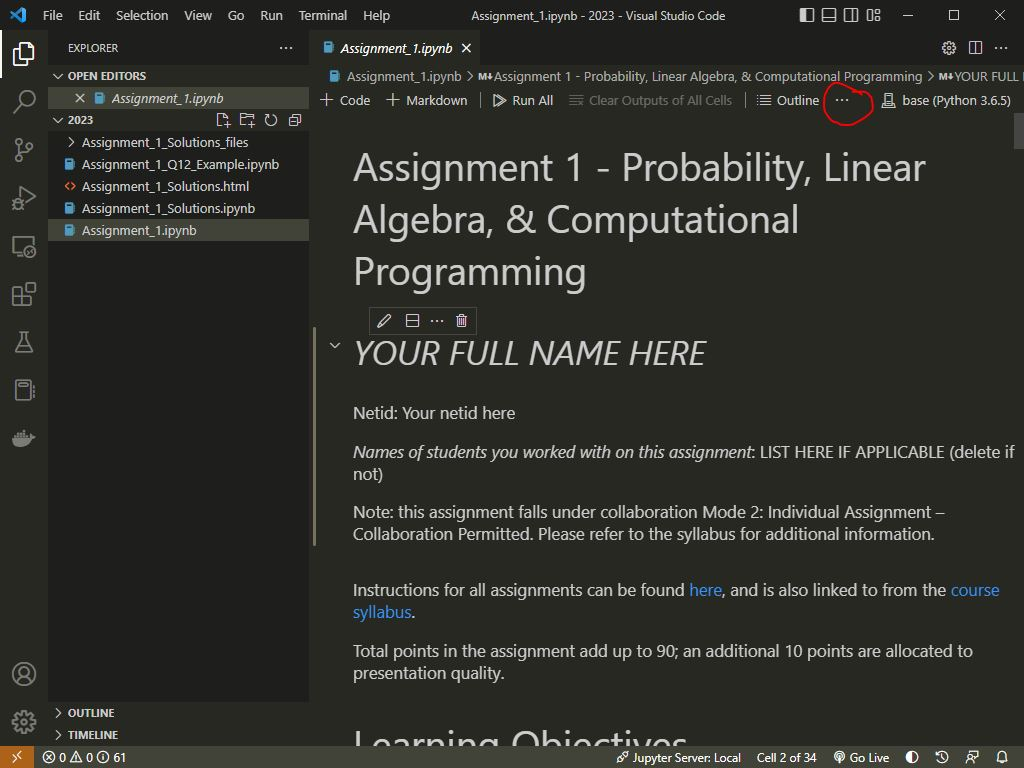
\includegraphics[keepaspectratio]{images_instruction/guide01.JPG}}

\begin{enumerate}
\def\labelenumi{\arabic{enumi}.}
\setcounter{enumi}{1}
\tightlist
\item
  Click ``Export'':
\end{enumerate}

\pandocbounded{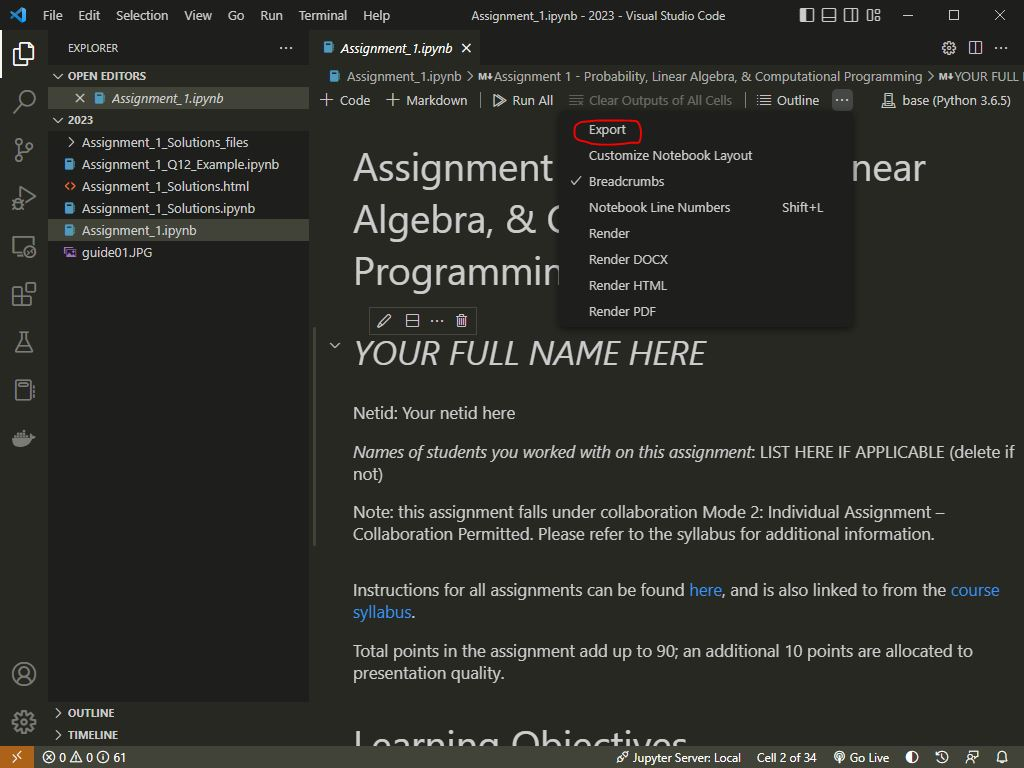
\includegraphics[keepaspectratio]{images_instruction/guide02.JPG}}

\begin{enumerate}
\def\labelenumi{\arabic{enumi}.}
\setcounter{enumi}{2}
\tightlist
\item
  Select ``HTML'' (exporting to pdf won't work without the installation
  of additional tools):
\end{enumerate}

\pandocbounded{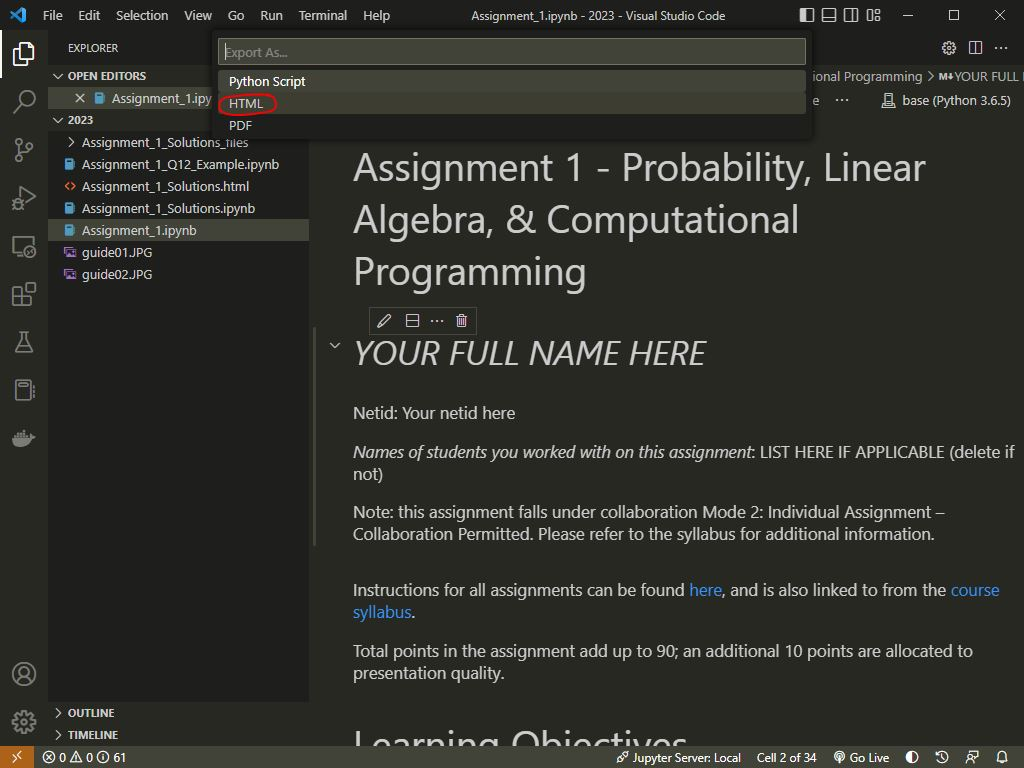
\includegraphics[keepaspectratio]{images_instruction/guide03.JPG}}

\begin{enumerate}
\def\labelenumi{\arabic{enumi}.}
\setcounter{enumi}{3}
\tightlist
\item
  Open the HTML file you just saved in Chrome:
\end{enumerate}

\pandocbounded{
\includegraphics[keepaspectratio]{images_instruction/guide04.JPG}}

\begin{enumerate}
\def\labelenumi{\arabic{enumi}.}
\setcounter{enumi}{4}
\tightlist
\item
  Click the options button (three vertical dots) and click ``print'':
\end{enumerate}

\pandocbounded{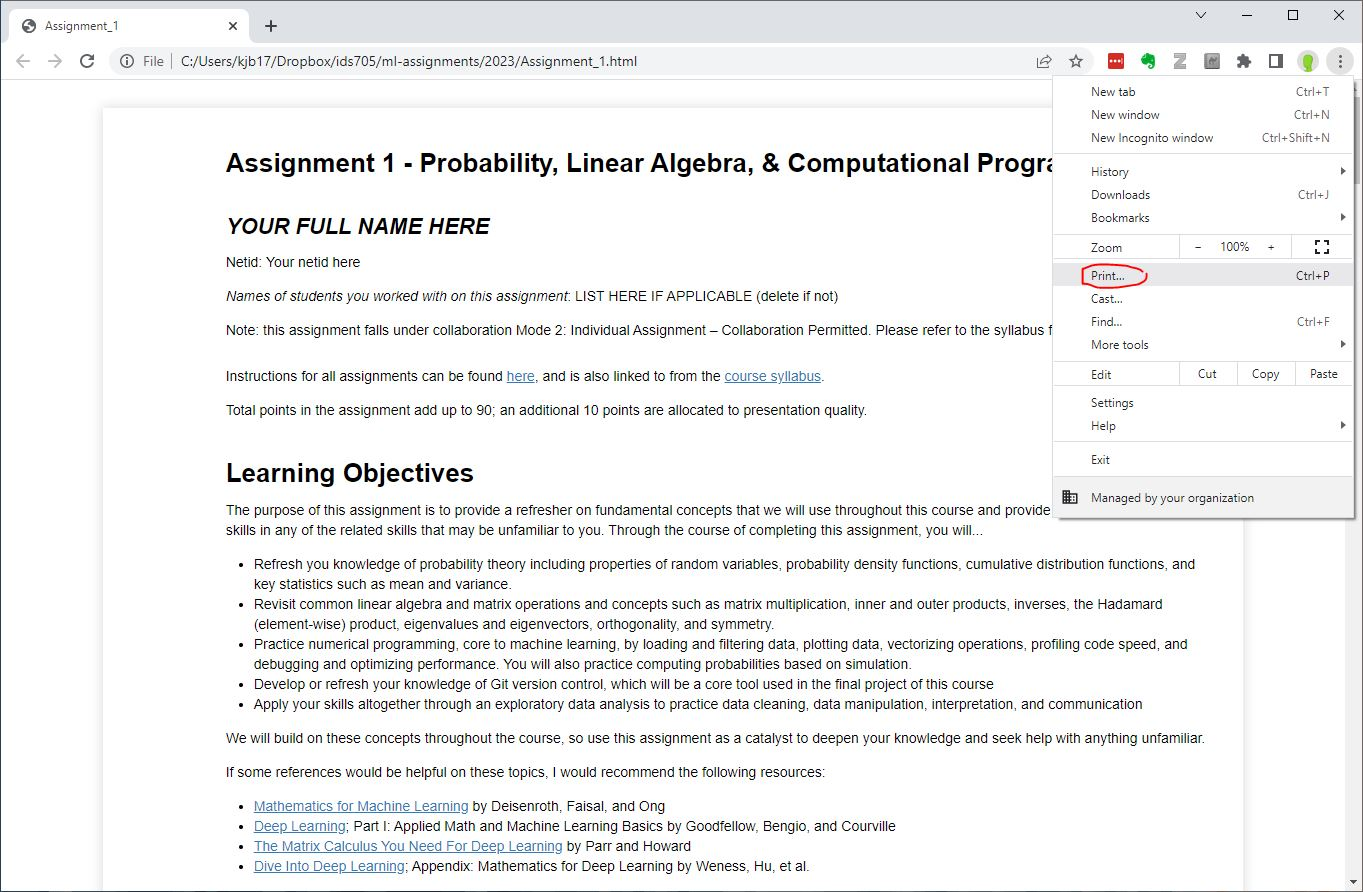
\includegraphics[keepaspectratio]{images_instruction/guide05.JPG}}

\begin{enumerate}
\def\labelenumi{\arabic{enumi}.}
\setcounter{enumi}{5}
\tightlist
\item
  Select the destination as ``Save as PDF'' and click ``Save'':
\end{enumerate}

\pandocbounded{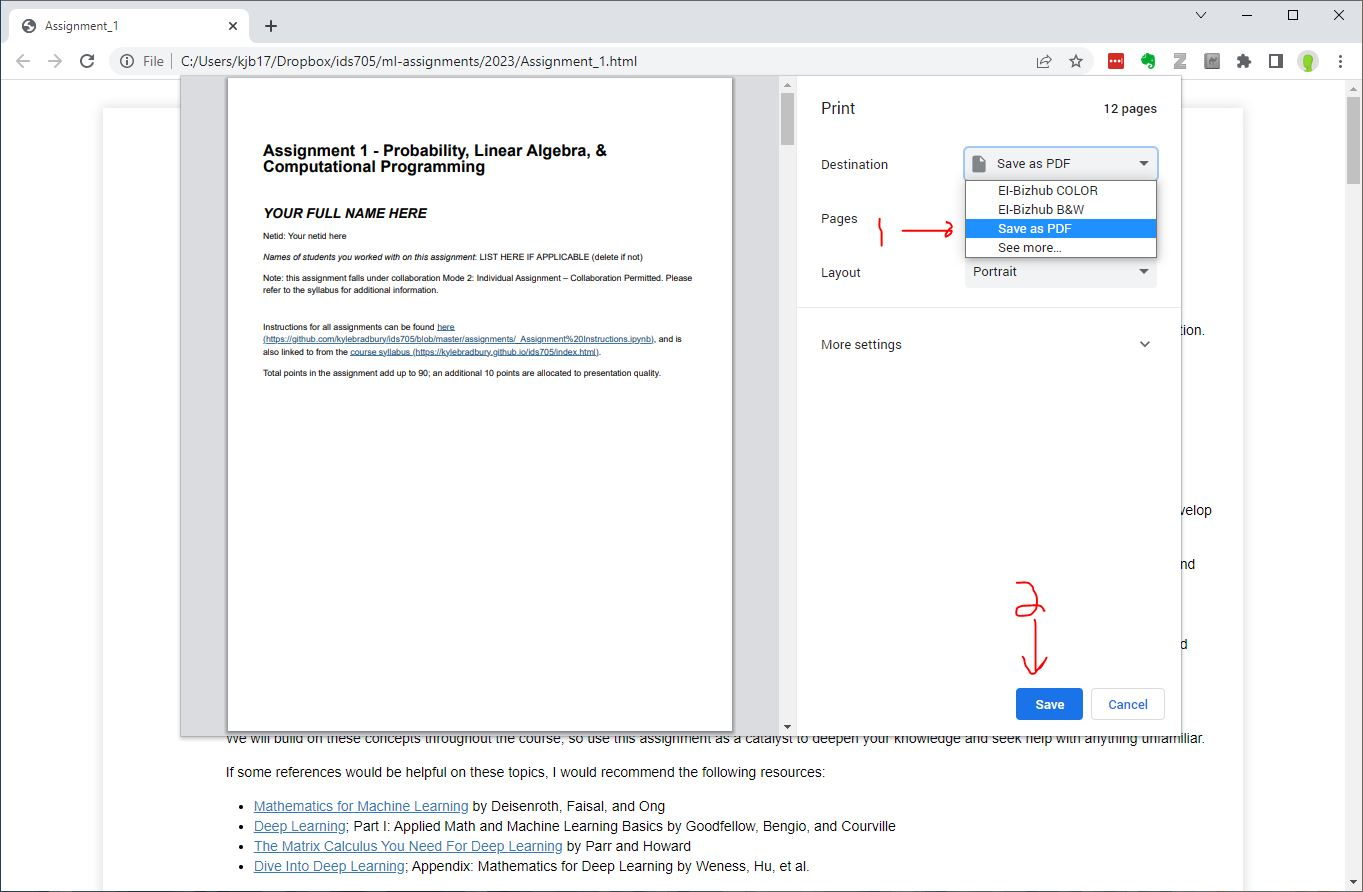
\includegraphics[keepaspectratio]{images_instruction/guide06.JPG}}

\begin{enumerate}
\def\labelenumi{\arabic{enumi}.}
\setcounter{enumi}{6}
\tightlist
\item
  Voila! You should have a pdf
\end{enumerate}

\subsubsection{Option 2: Render from VS Code with Quarto and
LaTeX}\label{option-2-render-from-vs-code-with-quarto-and-latex}

You can save a lot of the above steps if you're willing to install 2
things: 1. Install \href{https://quarto.org/}{Quarto}, which is an
open-source scientific and technical publishing system (great for making
websites and blogs for your professional portfolio). 2. Install the
Quarto VS Code extension 3. Install a
\href{https://nbconvert.readthedocs.io/en/latest/install.html\#installing-tex}{version
of tex} for your operating system. 4. Once you do this, you can directly
export your documents to pdf:

\pandocbounded{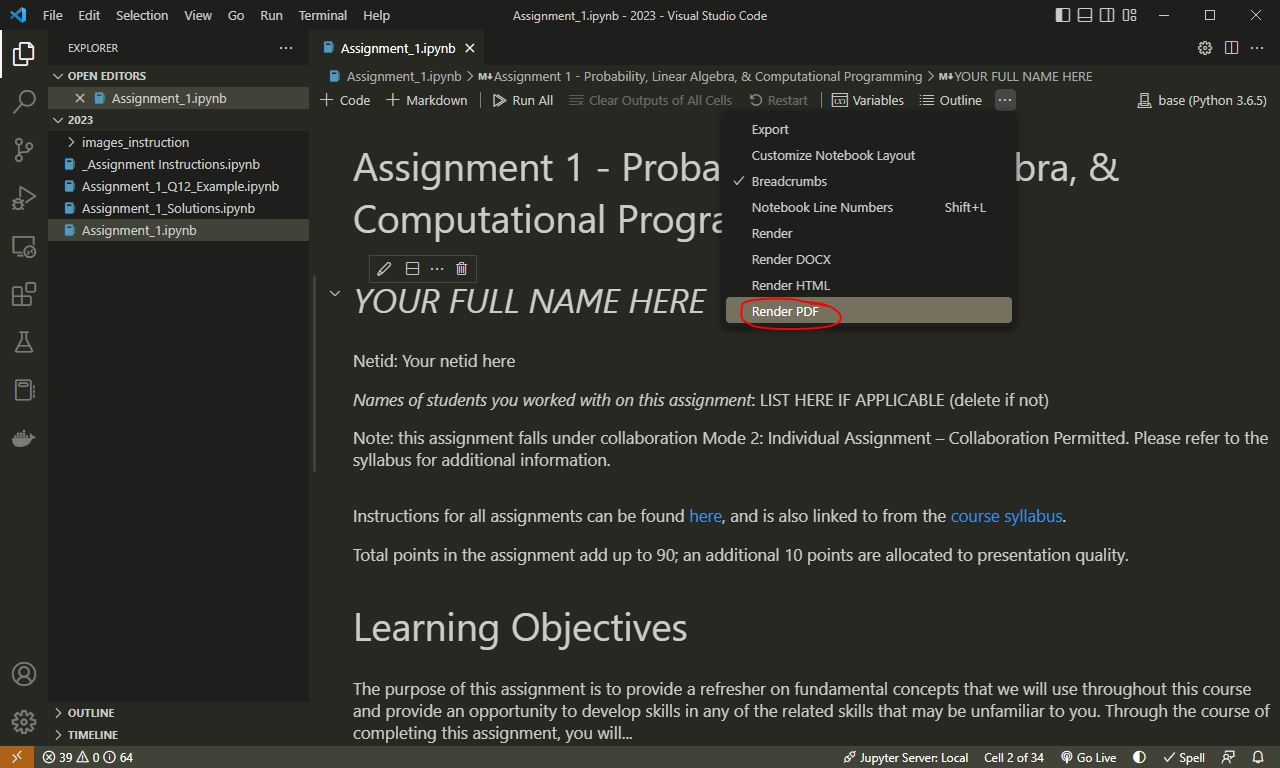
\includegraphics[keepaspectratio]{images_instruction/guide07.JPG}}

\subsubsection{Option 3: Render from Jupyter
Notebooks}\label{option-3-render-from-jupyter-notebooks}

Open your notebook in a Jupyter Notebook in Google Chrome. Go to
File-\textgreater Print Preview, then after verifying the document looks
correct, click ``print'' and for your printer choose ``Save as PDF.''

\textbf{Whichever method you choose - always check your pdf before
submitting to make sure everything is rendered and nothing is cut off!}

\subsection{Figure Guidelines}\label{figure-guidelines}

Here is an example of a well-prepared figure that checks all of the
requirements for good figures. Please check out
\href{https://www.coursera.org/learn/python-data-modeling}{this Coursera
course} for skill development and Python plotting best practices.

\subsubsection{Figure checklist}\label{figure-checklist}

\begin{enumerate}
\def\labelenumi{\arabic{enumi}.}
\tightlist
\item
  All plots should have a purpose - either being directly requested or
  should make a clear point.
\item
  \textbf{All} plots should have axes labels and legible fonts (large
  enough to read).
\item
  Legends are used when there are multiple series plotted on a single
  plot.
\item
  Markers on plots are properly sized (e.g.~not be too big nor too
  small) and/or have the appropriate level of transparency to be able to
  clearly read the data without obscuring other data.
\item
  If there are multiple colors used on a plot, EVERY color can be
  distinguished from the rest.
\item
  Figures are crisp and clear - there are no blurry figures.
\item
  Plots should be explained clearly in text or have a caption explaining
  them
\end{enumerate}

To demonstrate we'll start by loading some data to plot (the example
here is from the lecture on the bias-variance tradeoff):

\begin{Shaded}
\begin{Highlighting}[]
\ImportTok{import}\NormalTok{ numpy }\ImportTok{as}\NormalTok{ np}
\ImportTok{import}\NormalTok{ matplotlib.pyplot }\ImportTok{as}\NormalTok{ plt}
\ImportTok{import}\NormalTok{ pickle}

\CommentTok{\# Load the data for plotting}
\NormalTok{datafilename }\OperatorTok{=} \StringTok{\textquotesingle{}./plot\_example\_data/data.pkl\textquotesingle{}}
\NormalTok{infile }\OperatorTok{=} \BuiltInTok{open}\NormalTok{(datafilename,}\StringTok{\textquotesingle{}rb\textquotesingle{}}\NormalTok{)}
\NormalTok{loaded\_data }\OperatorTok{=}\NormalTok{ pickle.load(infile)}
\NormalTok{infile.close()}

\CommentTok{\# Store the loaded data in convenient variable names}
\NormalTok{kvalues }\OperatorTok{=}\NormalTok{ loaded\_data[}\StringTok{\textquotesingle{}kvalues\textquotesingle{}}\NormalTok{]}
\NormalTok{error\_training }\OperatorTok{=}\NormalTok{ loaded\_data[}\StringTok{\textquotesingle{}error\_training\textquotesingle{}}\NormalTok{]}
\NormalTok{error\_testing }\OperatorTok{=}\NormalTok{ loaded\_data[}\StringTok{\textquotesingle{}error\_testing\textquotesingle{}}\NormalTok{]}
\NormalTok{error\_bayesclf }\OperatorTok{=}\NormalTok{ loaded\_data[}\StringTok{\textquotesingle{}error\_bayesclf\textquotesingle{}}\NormalTok{]}

\CommentTok{\# Choose colors that will be distinguishable from one another}
\NormalTok{color0 }\OperatorTok{=} \StringTok{\textquotesingle{}\#121619\textquotesingle{}} \CommentTok{\# Dark grey}
\NormalTok{color1 }\OperatorTok{=} \StringTok{\textquotesingle{}\#00B050\textquotesingle{}} \CommentTok{\# Green}
\NormalTok{color2 }\OperatorTok{=} \StringTok{\textquotesingle{}\#7c7c7c\textquotesingle{}} \CommentTok{\# Light grey}
\end{Highlighting}
\end{Shaded}

Then, we create the plot:

\begin{Shaded}
\begin{Highlighting}[]
\OperatorTok{\%}\NormalTok{config InlineBackend.figure\_format }\OperatorTok{=} \StringTok{\textquotesingle{}retina\textquotesingle{}} \CommentTok{\# Make clear on high{-}res screens}

\CommentTok{\# Create the plot}
\NormalTok{fig, ax }\OperatorTok{=}\NormalTok{ plt.subplots(figsize}\OperatorTok{=}\NormalTok{(}\DecValTok{7}\NormalTok{,}\DecValTok{5}\NormalTok{), dpi}\OperatorTok{=} \DecValTok{100}\NormalTok{) }\CommentTok{\# Adjust the figure size and dots per inch to make it legible and clear }
\NormalTok{ax.semilogx(kvalues,error\_training,}
\NormalTok{            color}\OperatorTok{=}\NormalTok{color0,}
\NormalTok{            label}\OperatorTok{=}\StringTok{\textquotesingle{}Training (in{-}sample)\textquotesingle{}}\NormalTok{)}
\NormalTok{ax.semilogx(kvalues,error\_testing,}
\NormalTok{            color}\OperatorTok{=}\NormalTok{color1,}
\NormalTok{            label}\OperatorTok{=}\StringTok{\textquotesingle{}Test (out{-}of{-}sample)\textquotesingle{}}\NormalTok{)}
\NormalTok{ax.semilogx(kvalues,error\_bayesclf,}\StringTok{\textquotesingle{}{-}{-}\textquotesingle{}}\NormalTok{,}
\NormalTok{            color}\OperatorTok{=}\NormalTok{color2,}
\NormalTok{            label}\OperatorTok{=}\StringTok{\textquotesingle{}Bayes (optimal)\textquotesingle{}}\NormalTok{)}
\NormalTok{ax.legend()}
\NormalTok{ax.grid(}\StringTok{\textquotesingle{}on\textquotesingle{}}\NormalTok{)}
\NormalTok{ax.set\_xlabel(}\StringTok{\textquotesingle{}k nearest neighbors\textquotesingle{}}\NormalTok{) }\CommentTok{\# Always use X and Y labels}
\NormalTok{ax.set\_ylabel(}\StringTok{\textquotesingle{}Binary Classification Error Rate\textquotesingle{}}\NormalTok{)}
\NormalTok{ax.set\_xlim([}\DecValTok{1}\NormalTok{,}\DecValTok{200}\NormalTok{]) }\CommentTok{\# Ensure the axis is the right size for the plot data}
\NormalTok{ax.set\_ylim([}\DecValTok{0}\NormalTok{,}\FloatTok{0.5}\NormalTok{])}
\NormalTok{fig.tight\_layout() }\CommentTok{\# Use this to maximize the use of space in the figure}
\NormalTok{plt.show()}
\end{Highlighting}
\end{Shaded}

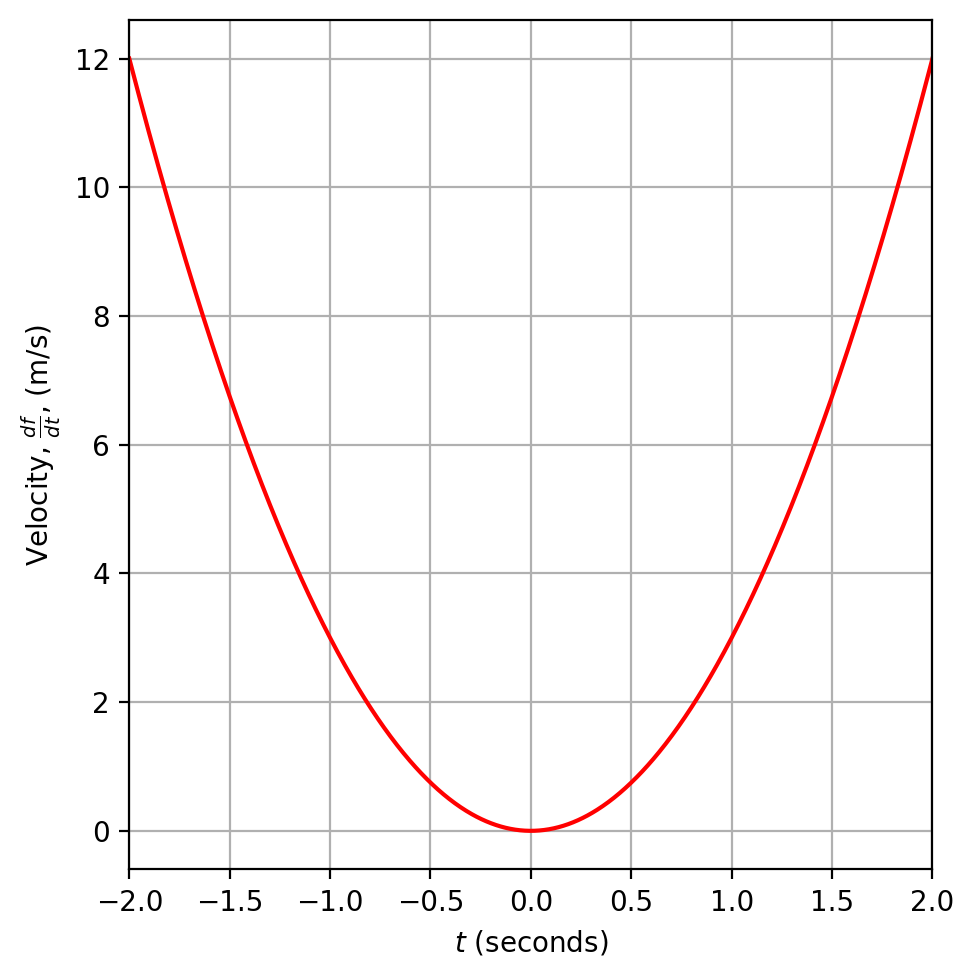
\includegraphics[width=7.17708in,height=5.0625in]{assignment_instructions_files/figure-pdf/cell-3-output-1.png}

\emph{Figure 1. Ideally, each figure should have a caption that explains
the figure. Here, the test data (green) approximates the generalization
error rate, the lower-bound of which is the Bayes error rate (grey
dotted line). The value of \(k\) represents the flexibility of the model
with lower values of \(k\) representing higher model flexibility and
higher values of \(k\), lower flexibility. The training error (black) is
not considered out of sample, so in cases of high model flexiblity (and
in this case high overfit), the training error rate can reach zero.}

Note the clear x and y axis labels and legends - there are no acronyms
or shorthands used, just the full description of what is being plotted.
Also note how easy it is to compare the color of lines and identify the
baseline (Bayes) comparison line. Make your plots easy to read and
understand. A figure caption is generally helpful as well to indicate
what we are seeing in each plot.

\subsection{Sources}\label{sources}

\emph{Some questions on the assignments are adapted from sources
including}:\\
1. James et al., \emph{An Introduction to Statistical Learning}\\
2. Abu-Mostafa, Yaser, \emph{Learning from Data}\\
3. Weinberger, Kilian, Machine Learning CS4780, Cornell University




\end{document}
